\documentclass[11pt, a4paper]{article}

\usepackage{mlt-thesis-2015}

% With Xetex/Luatex this shouldn't be used
%\usepackage[utf8]{inputenc}

\usepackage[english]{babel}
\usepackage{graphicx}
\usepackage{setspace}
\usepackage{float}

\title{Embodied question answering in robotics environment}
\subtitle{Automatic generation of a synthetic question-answer data-set }
\author{}

\begin{document}

%% ============================================================================
%% Title page
%% ============================================================================
\begin{titlepage}

\maketitle

\vfill

\begingroup
\renewcommand*{\arraystretch}{1.2}
\begin{tabular}{l@{\hskip 20mm}l}
\hline
Master's Thesis: & 30 credits \\
Programme: & Master’s Programme in Language Technology\\
Level: & Advanced level \\
Semester and year: & Spring, 2020\\
Supervisor & ()\\
Examiner & ()\\
Report number & (number will be provided by the administrators) \\
Keywords & (Artificial Intelligence,  Natural Language Processing, Computer Vision, Visual Question Answering, Synthetic Data-sets  ) 
\end{tabular}
\endgroup

\thispagestyle{empty}
\end{titlepage}

%% ============================================================================
%% Abstract
%% ============================================================================
\newpage
\singlespacing
\section*{Abstract}
    Our work extends a dataset for Embodied-Question-Answering. Embodied question answering is the task of asking a robot a question about objects in a 3D environment, where the agent is expected to navigate the environment and find the entities in question and answer. The answer system consists of navigation and VQA components.  Each question in the dataset is an executable function that could be run in the environment to yield an answer.  The published dataset for EQA is EQA-V1, and it is a limited dataset that includes only two types of questions, color and location questions. We use the navigational data, required for training the system, from EQA-V1 and generate new questions of two more types, size and spatial questions. Our data extension is intended to better train the system and enhance its ability in performing the task. 

\thispagestyle{empty}

%% ============================================================================
%% Preface
%% ============================================================================
\newpage
\section*{Preface}

Acknowledgements, etc.

\thispagestyle{empty}

%% ============================================================================
%% Contents
%% ============================================================================
\newpage

\begin{spacing}{0.0}
\tableofcontents
\end{spacing}

\thispagestyle{empty}

%% ============================================================================
%% Introduction
%% ============================================================================
\newpage
\setcounter{page}{1}

\section{Introduction}
\label{sec:intro}

An intelligent robot must be able to understand and resolve references in its environment (\cite{russell1995artificial}). Our human ability to interact in reference to our visual surroundings, manifested in language, stems from faculties such as perception and memory(\cite{regier1996human}). Perception, in particular, is central to our physical experience of the world (\cite{barsalou1999perceptual}). We conceive the physical world through perception; and we express our conceptualization of the perceptual experience in words(\cite{lakoff2008metaphors}). Therefore, the exhibition of intelligent behaviour is necessitated by having a notion of meaning that associates 'words' with the visual/physical world(\cite{nilsson2007physical}). 

\subsection{meaning}

The  meaning of words is not a mere psychological phenomena. Concrete nouns,for example, have references in the physical world, with physical properties indicated by their meaning. The meaning of a word, is, thus, not only bound up with linguistic characters and mental notion but also with some physical representation in the world. For example, the word "chair" is represented by its token-characters (c,h,a,i,r), contains a perceptual symbolism(mental understanding of the chair's attributes and functions), and refers to an entity with physical features in the world(\cite{mooney}).

In this triangular definition of meaning, vision has an integral part of meaning in which it represents the physical world to language. To recognize a chair, one should, for example, identify the existence of legs, seats, its sizes and geometric shape in a visual scene. These properties of the physical reference of a chair can be clearly represented in a visual form. Therefore visual recognition is part of the conceptualization process that form the perceptual symbol of an entity.(\cite{barsalou1999perceptual})

Perceptual information, however, is more than just visual information. The properties of an object includes other sensory information such as the smell, taste, and texture of an object. For example the meaning of rotten food could be more understood if the food is tasted. 

The formation of a symbolic representation (meaning) requires more than the recognition of perceptual information. The construct of a meaning (symbol) could only be formulated by the existence of knowledge about the relations of the attributes that form an entity.(\cite{barsalou1999perceptual}) refers to the process of forming a symbol as 'componential' or schematic, meaning that a  notion of meaning is a scheme that is logically constructed.

The full meaning is the perceptual representation and the knowledge about it. The meaning of rotten apple is fully understood when we construct a knowledge of the negative aspects of eating it. For example, rotten apples have red-brown colors, and the stomachache that result by eating them leads us to form the  belief that red-brown apples are different from all-red apples, not only by color but also other health/taste attributes, so we classify red-brown apple in different category called "rotten apples". The knowledge about health implications, and the attributes such as colors and smell of a rotten apple help us categorizing the rotten apple in the category of rotten food. (\cite{lakoff2008metaphors}) explains that this attributive characterization can be expressed, for example, in the way we do prototyping and categorization of entities.


\begin{figure}[H]
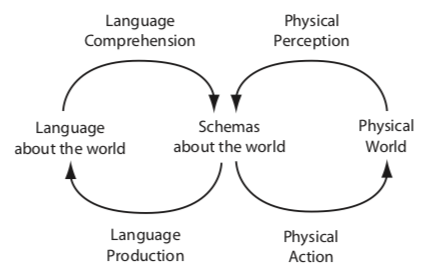
\includegraphics[scale=0.3]{images/symbolsyststem.png}
\caption{\cite{roy2005semiotic}}
\label{roy}
\end{figure}.

Interactions in the semantic world  has an exchangeable nature. The interaction allows us to form meaning and the formed meaning shape our language and actions. In \ref{roy} we see that the outcomes of our interaction in the world includes not only linguistic implications but also affects the actions(\cite{roy2005semiotic}). 'schemes about the world' are the beliefs we make from the interactions. For example, our negative experience with the red-brown apple made us form the  "belief" that rotten apples are bad. The knowledge of "rotten apples are bad" influence our future actions- makes us not eat the apples with attributes of "rotten". 

The process of comprehending meaning by means of associating attributes with each other to form a belief or draw a conclusion denotes the notion of reasoning. The process of classifying the apple as rotten includes multiple abstractions. We might first identity the apple by its general shape structure, then recognize, from previous experiences, that  apples in red-brown color is not like all-red apples then conclude that the apple is rotten. Reasoning is the ability to take the logical steps to come to a conclusion.  
 


\subsection{Grounding meaning}

The approaches to ground meaning(form meaning) varies dependent on the aspect of meaning that each approach focuses on. The different methods we review below approach meaning as a mental notion, a map of connected knowledge nodes,  vision and language representation or  the combination of different aspects of meaning representation. 


Word-meaning in a Vector Semantic Space (VSM) represents a mental aspect of meaning notion(\cite{Turney_2010})). Space can be understood by imagining our minds as a space that we allocate meaning representation in them. In VSM the mind (represented as neural language model) is an artificial space where word meanings are allocated at different distances from each other depending on their categorization, such as a rotten apple is closer to fresh apples than to chair. 

There are multiple hypothesis to representing word-meaning in a Vector Semantic Space(VSM). Distributional hypothesis is a popular example of word-representaion in VSM. The premise of this approach is that language is compositional and word-meaning can be defined by its context--The meaning of a word is represented by the word and the words surrounding it \cite{Turney_2010}. The formulated word meaning representation is known as "word-embeddings" \cite{mikolov2013distributed}. Using language to define language proven good in inferential tasks such as inferring that "university" and "student" are close to each other given their common context of "education". 
 
 
Representing meaning with a combined linguistic and visual representation is a second example of a field that is extensively researched. Early research in combining vision and language used probabilistic learning by aiming at drawing an alignment between sentences, phrases, and words with the corresponding perceptual representations.\cite{790410}. An approach  to probabilistic learning estimates the probability of a grammatical entity(text) being related to a perceptual representation \cite{6751319}. A second probabilistic method is by classifying each word in a sentence through probability distribution of words over a perceptual representation. In \cite{matuszek2012joint} \cite{larsson2015formal} we see examples of connecting entities of formal semantics(First Order Logic) with perception. 

Finally there are examples of research that attempt to incorporate knowledge graphs in the the representation of meaning. Examples, \cite{zhu2015building}, \cite{zhu2014reasoning}

Despite the variety of methods in forming meaning, the comprehension of a full meaning cannot be formed in exclusion of any of its aspects. Even abstract concepts can sometimes have a physical/visual representation such as Art. Art works cannot be understood if we do not perceptually perceive them and connect them to some mental notion of knowledge. In order to achieve such high cognition abilities in robots, scientist and researchers are continuously introducing finding new methods and approaches to improve the computer's abilities.  

In  robots, a full comprehension of meaning is essential for its usability. 
the ability to understand the visual aspect of meaning is essential for the robot's ability to interact and preform action. 

A paragraph about neural language models for vision and language (intro for image captioning)






%\cite{dunning1993} introduced a well-known method for extracting
%collocations. Bilingual data can be used to train part-of-speech
%taggers \citep{das2011}. Another one: \citep{cortes2014}

Testing Unicode: Göteborgs universitet

\textit{Testing} \textbf{testing} \textsc{testing} some font series.

Testing a formula:
\[
P(X) = \sum_{i=1}^N P(A_i) P(X|A_i)
\]

Testing a table:
\begin{table}[htbp]
\begin{center}
\begin{tabular}{c|c}
cell 1 & cell 2 \\
\hline
cell 3 & cell 4
\end{tabular}
\caption{This is a table.}
\end{center}
\end{table}



\newpage

\section{background}
\label{sec:background}







\subsection{image captioning}

Image captioning is an extensively researched field where visual-grounding is at the  center of its focus. The methods of image captioning provide insights helpful for tasks that combine vision an language. In this section we review two main methods used in image captioning,feature extraction and attention mechanisms.   

Video \cite{Lin2014VisualSS}


\subsubsection{Feature extraction-CNN+RNN}

Feature extraction methods can be divided into two main groups. The first group relies on statistical language models(described in the previous section as transparent function). The second group relies on encoder-decoder neural network model that deep extracts features.\cite{Imagecap}

\paragraph{Encoder-Decoder(CNN-RNN)}



Convulutional neural networks are at the core of feature extraction methods. CNN applications, nonetheless, take a vital role in many computer vision tasks. We see CNN and its modified models (such as recurrent-CNN) used in tasks as object recognition \cite{liang2015recurrent} \cite{objdet} \cite{Ren2015FasterRT} , image classification \cite{simonyan2014very} \cite{imclassfication},and  semantic segmentation \cite{hariharan2015hypercolumns} \cite{imseg}. 

The reason for using CNN for image processing  is its ability to reduce the high dimensionality of images. Image features contain large sizes represented in pixels which would require large number of parameters to train. CNN reduces the dimensions of an image by learning how to process a matrix from a large window such as 250x250 pixels into a smaller one as 25x25. Through computing the convolution values of the image matrices and executing pooling computations, this process reduces the image into a smaller representation. The latter reduces the computational load and helps in processing and classifying the images faster.   


The encoder-decoder caption generation has a CNN encoder and an RNN decoder.\cite{vinyals2015tell} is an example of an end-to-end neural captioon generation model. In the neural model the CNN process the image features, and the last hidden layer passed to an RNN to generate a description. This method is a sequence modeling that is similar to machine translation. This means that image features are translated into words. The sequence is predicted by finding the probability of a certain description from a corpora given the features of an image. 

RNN are known to be used widely in language technology applications. Rnn is used , for example in  text-to-speech \cite{arik2017deep} and  machine-translation \cite{cho2014learning},\cite{Wu2016GooglesNM}. The advantage that the RNN gives to these tasks is that the output size is not fixed and that each output depends on the previous one. Such an incremental-sequence prediction is suitable for sentence predictions in respect to word dependency.  

RNNs have a issue of vanishing gradient-descent. The gradient descent is an optimization algorithm that minimizes the error calculated in the loss function. Optimization, in brief description, is important for the learning process. It updates the model's parameters which determines the  direction taken in the next time-step. This information is calculated given the input-output and the values of the parameters from the previous time-stamps. The gradients is reduced at every step due the value deductions in the activation function. When the gradient is reduced to almost zero value, it will be updating the parameters with no useful values, and therefore, learning seizes to improve. 

Long-Short-Memory network (LSTM)  provides a good alternative for avoiding the disappearing gradient. The gradient in RNNS vanishes in long sequences where the gradient keeps reducing. The architecture of the LSTM allows it to keep information stored for very long sequences. The latter gives it the ability to control the values of the gradient by updating it with information stored in the 'forget gate' form previous steps, preventing the gradient from vanishing.  



\paragraph{Feature extraction- statistical language model}

Statistical language model, as in \cite{fang2015captions}, generate descriptions in three stages. First it detects words in an image using a convolutional neural network (CNN) for extracting image features. The incorporation of language at this stage happens using multi-instance learning(MIT)\cite{zhang2005multiple}. The second stage, the statistical language model detects the most likely sentence to make of the words from a pre-defined corpus. In the third stage the sentences undergoes a re-ranking stage where the sentences are combined to generate captions. 


\paragraph{Attention-mechanisms}


In the previous section the discussion on the methods and implementation 

\subsection{Dialogue and VQA}

In this section of the text we discuss the capabilities of computers to exhibit more intelligent behaviour. Image-captioning and its methods showed an insight to how much computers could see and understand what its seeing. However, acquiring language in the visual world would require computers to be able to communicate what it sees. Otherwise, in order to say that a computer is visually or linguistically intelligent one should imagine the computer having to pass the Turing test in a visual surrounding. 

Researchers attempt to improve systems that are capable to hold a dialogue with a visual content.\cite{das2017visual} trains a system in  encoder-decoder model on a data set of 2 pairs dialogue with an image content.\cite{Skoaj2011ASF} trains a system on learning concepts with visual content in an interactive-learning approach. 

To make a true statement about the computer's capability to engage in a visual dialogue, it must be first ensured that the computer actually understands the questions being asked to it. Otherwise, dialogue is very complex with many elements determining it succession. In a dialogue with visual content, the computer must, furthermore, understand the questions within their visual context. It is reasonable that we see increasing research on "Visual Question Answering" and less on visual dialogue as a whole. Improvements in VQA intuitively means that we are moving closer in the direction of having an interaction with a computer in a visual dialogue.  


 \cite{VQA} is the first notable data-set published for Visual Question answering (VQA). The data-set consist of open-ended and free-form questions. The data contains 250,207 images from MS COCO \cite{lin2015microsoft} and other abstract scenes.The question types in the dataset require a range of different capabilities such as common-sense reasoning, knowledge-based reasoning, object-detection and active recognition.
 
 Data-sets that use MS COCO scenes such as \cite{gao2015talking}, \cite{yu2015visual} in addition to \cite{VQA} used human workers to write the texts for the scenes. Other data-sets are generated automatically such as \cite{ren2015exploring}. 


\cite{zhu2016visual7w} introduces a  unique QA data-set. The Visual7W consist of questions about an image with objects marked with regions in the image. Object grounding with image region introduced in \cite{krishna2016visual} contains the largest data-set with regions for both VQA and Image-captioning. Object-region approach is intended to improve visual grounding, by marking the regions of the image that the strings refer to.

restricted visual Turing test to evaluate visual understanding. The DAQUAR dataset is the first toy-sized QA benchmark built upon indoor scene RGB-D images. Most of the

\subsection{Embodied Question Answering}

\begin{figure}[H]
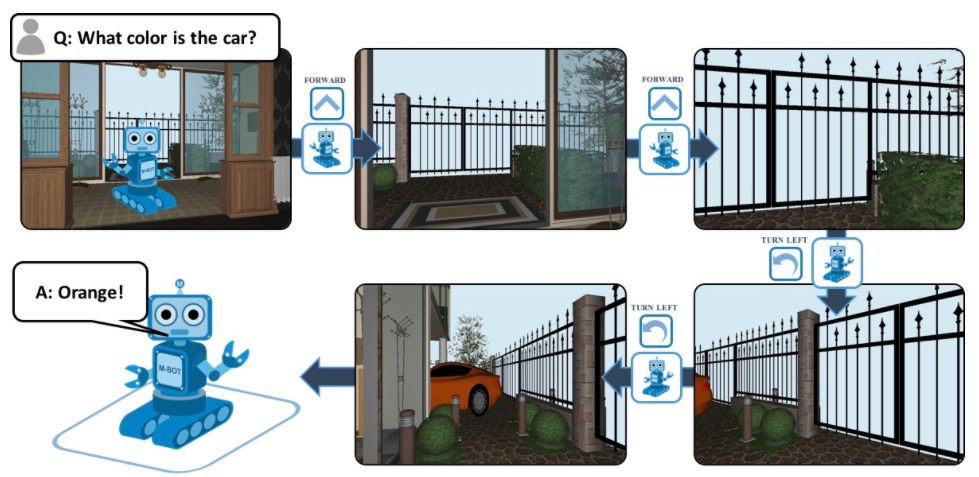
\includegraphics[scale=0.4]{latex/images/EmbodiedQuestionAnswering.png}
\label{fig:EQA}
\caption{The Robot is asked a question at a start position. It needs to look a round, collect information and decide on the next step to take. When it recognizes the car it stops and processes the scene to answer the question }
\end{figure}. 

Embodied Question Answering is a new interactive task presented as one of the tasks within the Habitat Platform\cite{embodiedqa}. The idea of the task is to allocate an agent at a random position in an  3D environment and ask it a question. To answer the question, the agent must intelligently explore the environment, collect information, and successfully navigate to the entity in question. EQA system navigates based on common reasoning, through an egocentric view, more or less imitating humans, it should be able to answer itself the common questions of “where am I?”, “where to go next?” and if asked a question about the car, as seen in \ref{fig:EQA}, it should be able to reason that cars are usually situated outside or in the garage and look for the exit. Once it navigates successfully to a point where it recognizes the car, the robot should stop and answer the question.  


\begin{figure}[H]
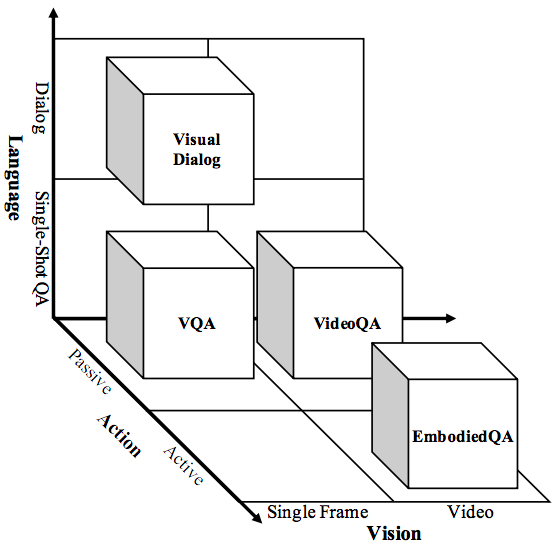
\includegraphics[scale=0.3]{images/Vision-language.png}
\caption{EQA in relation to other multi-modalitied  }
\ref{fig:multimodal}
\end{figure}.


 EQA shares some common ground with other multi-modality tasks of vision and language but is distinguished by other functionality. In figure \ref{fig:multimodal}  (paragraph to be written)



The novelty of this system is that it presumably solves a problem of navigating and performing tasks in unseen environments. Many of the earlier studies that deal with navigation such as \cite{kruijff2007situated}\cite{lauria2001training} require the system to have a localized map of the environment in order to be able to navigate in it. The problem of localization in robotic navigation is known as Simultaneous Localization and Map Building(SLAM). SLAM is a problem where a robot should be able to  map an unknown environment without a GPS or local map. Simultaneous localization is when a robot discover its surrounding and simultaneously construct a map while aware of its changing location. This means that the robot should extract information from its surrounding and learn the map as it goes \cite{grisetti2010tutorial} \cite{938381} \cite{8482266}. 



The answering system in the robot consist of two components. The first is navigation, and the second is Visual Question Answering. The navigator is responsible for navigating to the scene ... The agent needs to successfully navigate to the target object. Once the agent reaches the goal it would stop at the target location and would process the question and the visual input to answer the question.




In order to implement the whole embodied question answering we can say that the system consists of multiple combined parts, such as vision, navigation, reasoning and answering. However,the design of the system allows it to exclusively perform visual question answering on the baselines, without training and testing the navigation. The evaluation is done on the model that is responsible for question-answering at the scene point where the target object exists.Therefore, before discussing any other related constructs in the Habitat platform, such as agent, working flow, it is important to first look at the part of the system that this paper aims to evaluate. 









\subsubsection{navigation}



Habitat's navigation is referred to as PACMAN. It consist of two core components, planner and controller. The planner takes inputs from the vision and language model, and the encoding of hidden-layer and action of the previous time-step , then outputs action-decision. 

\begin{figure}[H]
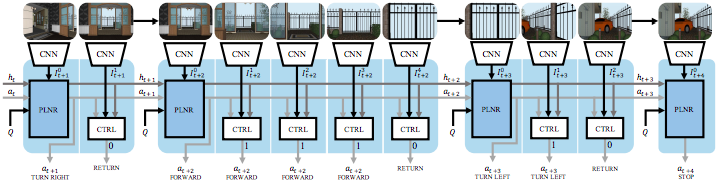
\includegraphics[scale=0.53]{images/nav.png}
\caption{}
\label{fig:nav}
\end{figure}

The controller takes the previous hidden state and action-decision and executes the action. As seen in \ref{fig:nav}, visual input is passed to the control then the controller classify the next decision of two possible decisions. Either to repeat the last action given by the planner or to return to the planner. The controller can repeat the same action maximum five times then it automatically returns to the planner. 

Visualization of the navigation is in figure (1). T stands for the planner's time-steps, t = 1,2,3...., and N(t),  n = 0,1,2,3.. denotes the controllers time-steps. The denotations of symbols explained clearer in the quotation : 


"\begin{math}  I_{t}^{n} \end{math}denote the encoding of the observed image at t-th planner-time and n-th controller-time. The planner is instantiated as an LSTM. Thus, it maintains a hidden state \begin{math} h^{t}\end{math}
(updated only at planner timesteps), and samples action 
\begin{math}  a_{t} \ \in \ \{forward,\ turn-left,\ turn-right,\ stop\} \end{math} "p(6)
\vspace{0.3cm}

For eample the first  step-decesion from the planner is denoted as such: 
\vspace{0.3cm}

\hspace{1cm}        \begin{math} a_{t} ,h_{t}{}\leftarrow PLNR\left( h_{t-1} ,I_{t}^{o} ,Q,a_{t-1}\right) \end{math},
        
\vspace{0.3cm}

The planner computes the next step-action  \begin{math} a_{t+1} \end{math} from input of the previous hidden layer \begin{math} (h_{t-1}) \end{math}, question encoding (Q), the previous action  \begin{math} a_{t-1} \end{math}, and the image input given to the PlNR \begin{math} (tI_{t}^{o}) \end{math}.The planner selects the action \begin{math} a_{t+1}\end{math} and update the hidden state \begin{math} h_{t+1} \end{math} then passes the control to the controller. 

\vspace{0.3cm}
(The basis of the controller decision is a bit unclear)

The controller decides to either repeat the action or return control to the planner. The controller's classification is based on the current hidden-state\begin{math} h_{t}  \end{math} and current action \begin{math} a_{t} \end{math} and the image observation from the planner + the image given at the controller's time-step. The denotation of the classification is as such: 

\vspace{0.3cm}

\[ \{0,1\} \ \backepsilon \ c_{n}^{t} \ \leftarrow CTRL\ \left( h_{t} ,a_{t} ,I_{t}^{n}\right)  \]

"if \begin{math} c_{n}^{t} = 1 \end{math} then the action \begin{math} a_{t} \end{math} repeats. Else \begin{math} c_{n}^{t} = 0 \end{math} or a max of 5 controller-times been reached, control is returned to the planner"p(6). The \begin{math} h_{t} \end{math}   \begin{math} a_{t} \end{math} coming from the planner act as an intent. The controller, initiated  as "feed-forward multi-layer perceptron with 1 hidden layer",repeats and controls the action in order to align \begin{math}  I_{t}^{n} \end{math} with intent given by the planner. 

\subsubsection{VQA Model}

\begin{figure}[H]
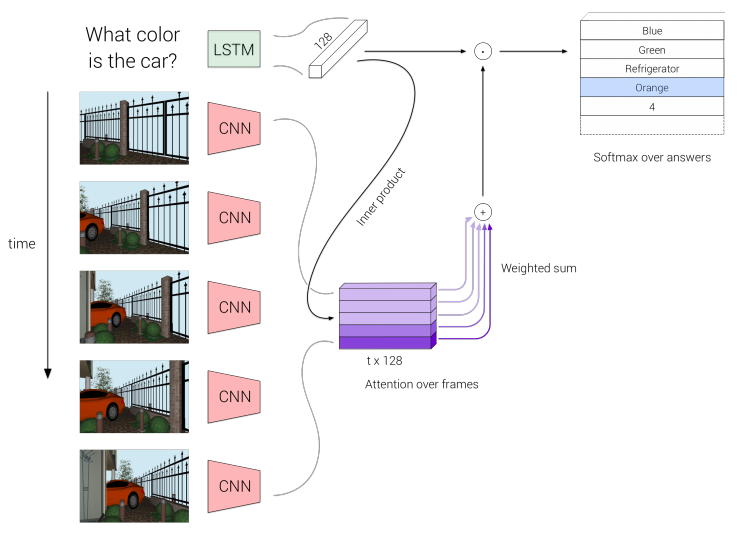
\includegraphics[scale=0.35]{latex/images/VQA.png}
\caption{}
\label{fig:VQ}
\end{figure}

(Text already exist .... To be completed)

The VQA model consists of two parts, one is a CNN model to extract features from the scene images(5 frames), and the other takes the question input and combine it with the wights of the images. Figure 1 illustrates the combination of the two parts. 





\subsection{Problem}



In an experiment we conducted on the VQA model, we noticed that the system tends to answer questions relying mainly on the questions (bias). The question of the experiment is if the answer-prediction would change or still be correct if we ask the system about the color of the table in the living room and input a picture of a bathroom without a table in it. \ref{}

The results showed an increase in the total accuracy of the prediction despite the absence of the required visual information.
 
 Yasmeen expirement {............}
 
 These results could indicate different things on the model and its data, but the least it could tell is that the system did not need to rely on the images to answer the questions correctly.

\subsubsection{dataset bias}
The observation of the results opens question-marks on two major components. The first is on the VQA model, as by why it tends to neglect the visual information and rely mostly on linguistic features. The second is a question on the dataset and its contribution to answering the questions correctly. Nonetheless, if one assumes that the model's ineffectiveness stems from a model-data mismatch, how would the system perform if asked different types of questions than the existing ones. This speculation becomes more relevant given that evaluated questions consist predominantly of one question type, color.



\subsection{Problem in a context}


In a more concrete example, a reasoning process would "require models to perform inference at multiple levels of abstraction" \cite{selvaraju2020squinting}. for example, "is the banana ripe?" where it would instantly answer "no".  To answer this question, it would require the system to rely on perception to answer sub-questions such as where is the object? What are its shape, size, and color? Then reason that the "yellow" color indicates ripeness.


A common problem in visual question answering is the over-weighting of linguistic over visual features in the answering. \cite{fukui2016multimodal}. Research has shown that models can superficially perform tasks without learning the underlying reasoning process \cite{turmsimple}. In visual question answering, it has been observed that a system cheats its way into answering the questions without taking the reasoning steps that humans would logically take to answer a question. \cite{agrawal2016analyzing},\cite{zhang2016yin}, \cite {fukui2016multimodal}.In particular, 

In Such cases the system answers correctly by exploiting linguistic biases in the dataset, as it tends to rely primarily on the language model and ignore the visual information \cite {goyal2017making}

model learns biases in training and manages to give good results in the testing \cite{selvaraju2020squinting}. The underlying issue here is that the model answers by memorising prior textual information. For example, a neural network might answer the question “What covers the ground?” correctly by answering “snow”, “not because it understands the scene but because biased datasets often ask questions about the ground when it is snow-covered.” \cite{johnson2017clevr}; This learning problem is crucial because it makes it challenging to evaluate the model’s improvements\cite{agrawal2018don}.


However, color questions could get more complex as "people employ compositional color descriptions to express meanings not covered by basic terms, such as greenish-blue" \cite{monroe2016learning}. It would be shallow to assume that color questions are simplistic, especially if we expect the system to answer colors beyond the basic color terms like "green" and "red." 


\subsection{Research Questions}



Research question: 

- How can we extend the data-set with more sophisticated and natural questions.
- What is the bias formed by color questions. 
- How does the VQA system preform with the new question type. 
- Does asking size and spatial question improve the system's attention to vision.  


- overview how habitat is constructed 

- Does asking more questions of size and spatial types improve the system's attention to vision?

- How does the system preform when we ask more question types?


We have an evidence that the dataset is simplistic, and contains bias in color question. (cause of the problem). problem- lack of visual grounding. 

- How does the system preform when we ask more question types?
- How does the 

questions. (A usful robot should answer a variety of questions.)

. To what extent does the system use  the visual information.

. Does asking more questions of size and spatial types improve the system's reliance on vision, rather than language.

. How would the navigation model preform with new questions. 


. Does the inclusion of spatial questions improve the system's learning of computational answers- such as olive-green, dark -blue. 

. Would a tranformer-based based attention model improve the the preformance of the vqa model. 

Adding new questions could help test the system's capabilities, but more importantly, we consider it a step to enhance the system's cognition. The VQA system that we are improving is part of a robotic system that should ideally be helpful for human use. Social robot's usability is very dependent on its exhibition of human intelligence \cite{fong2003survey}. Hence that correct question-answer prediction does not necessarily indicate the system's ability to reason. 

An example from the data presented in the Habitat project requires even fewer abstractions, "what color is the sofa?"; The system would only need to rely on perception answer itself "where is the object," then answer the color question.


\newpage

\section{Methods and materials}
\label{sec:methods}
\subsection{Habitat Simulator and Lab- Overview}

We use the Habitat platform as a host for the EQA task. The name 'Habitat' is derived from  the notion of learning within and from an environment. Imitating our natural habitat, the Habitat platform facilitates spawning an agent in a simulated environments with the possibility of teaching the robot to preform different tasks. 

The perquisites needed to test or train an agent for a certain task in a given environment, are facilitated by a core component called  Habitat Simulator. Habitat Simulator is responsible for simulating an  environment and insinuating a robot in it. The simulator acts depending on the configurations given to it. 

The configurations are processed into commands in Habitat-lab before being passed to the simulator. Habitat lab is the second core component of the system. In addition to giving commands to the simulator, the Habitat Lab module acts as a pipeline that prepares the data-set of the corresponding task. The habitat-lab module,in other words, is the coordinator that informs the simulator of the required setting, and the data loader and processor that prepares the data for either training or testing. 

\begin{figure}[H]
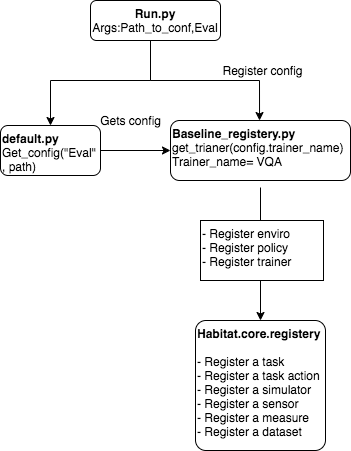
\includegraphics[scale=0.43]{images/configProcess.png}
\label{fig:configs}
\end{figure}

Figure(x) resembles a map of the code structure when the habitat lab module is initiated to preform a task. Each task has its own configurations and in this example the task is 'VQA evaluation'. As seen in the figure \ref{configs}, the module takes hierarchical steps in which each step is executed in accordance to the configuration of the given task. In the most down box of the structure we see parts of the commands directed for the simulator, such as insinuating an environment and sensors in the agent. Other commands include registering a data-set which takes part in lab module. 


Embodied question-answering is part of the tasks included within the Habitat platform. The EQA task consist of two sub tasks. The first is navigation, and the second is Visual Question-Answering. The main idea of the task is that agent needs to successfully navigate to the target object. Once the agent reaches the goal it would stop at the target location and would process the question and the visual input to answer the question. 


However, there is no available connected model that connects(Nav,VQA). The researches elaborate that the system preform poorly if the two modules put to work together and trained in reinforcement learning. Setting up the task in such a connected manner lead to distorted images and inaccurate view point of the object in question if the robots drifts off the path during navigation. "Noisy or absent views"  would confuse the question-answering model.

The current configuration for the EQA task separates the training for navigation and VQA. Imitation learning is used for navigation, and supervised learning for question-answering. the navigation is frozen when once it completes a navigational episode and is evaluated based on its steps following the shortest path to the objective. VQA model is evaluated based on the answers predicted.  

'shortest path' is used in the training sitting of both, the navigation and VQA. 'Shortest path' is a navigational path consisting of the shortest steps to take to reach a view point of where the object in question is located. With each question-answer in the EQA data-set we find one shortest path. Shortest paths are made by human workers. For navigation the system is trained on following the steps of the shortest path. For VQA the shortest path is used to capture the scene from the viewpoint at the end of the path.  

However, the navigation might go off the shortest path and seek to take more actions to reach the goal. This might lead to distorted images and inaccurate view point of the object in question. "Noisy or absent views"  would confuse the question-answering model.

The vision-language modalities are fine-tuned differently for navigation and QA. Navigation and VQA employ the vision and language modalities provided in the platform. However, each one of them use the two modalities with different configurations, such as the number of decoders for vision and  the times that the language encoder is used.  


\subsection{vision}

The vision of the system relies on egocentric 224x224 RGB images processed in CNN. The CNN encoding has the functionality of a “multi-task pixel-to-pixel prediction framework,” which consists of 4 {5x5 Conv, BatchNorm, ReLU, 2x2 Max-Pool blocks}, and they produce a fixed-size representation.“The range of depth values for every pixel lies in the range r0, 1s, and the segmentation is done over 191 classes”(p.11). (page,6). 

It  is possible to train the encoder-decoder on generating  three sensory information. The three decoders, which can also be referred to as sensors take the functionality of: 1) RGB reconstruction, 2) semantic segmentation, and 3) depth estimation. The latter sensors are used to obtain “object attributes (i.e., colors and textures), semantics (i.e., object categories), and environmental geometry (i.e., depth).” . 

In the baseline models, different tasks take different sensors.Not all the above-mentioned sensors are used in all the baseline tasks. Since navigation and VQA are trained and evaluated separately, we refer to them as separate "tasks". The two tasks in EQA take the following sensors: 

{Navigation}:  "depth" and "RGB". Depth sensor is essential for the agent's capability to navigate. With depth sensor it could estimate distances and avoid colliding with obstacles.  

{VQA}: The existent baseline VQA model uses the visual information with "RGB" data only. (No reason mentioned to why the other sensors are not used in the question-answering baseline module).  


\subsection{language model}

The language models is a 2-layer LSTM with 128d hidden layers. The language model's role is to encode the questions and produce a representation. The language-encoder is trained differently for the navigation and VQA. The encoder learns to focus on different strings for each task. Some words in the question can be crucial for executing one of the tasks while less useful for the other task. An example of a question, cited from the EQA paper, " ‘What color is the chair in the kitchen?’, ‘color’ is irrelevant for navigation and ‘kitchen’ matters little for question answering (once in the kitchen) "

%Hence- current hidden-state h_{t} and the current action are only %updated in the planner: 
%
%The controller executes the action  a_{t+1}. It takes then the 
%
%Hence, h_{t-1} and a_{t-1} carry no information at the 0 timestep %since no encoding or action been outputed by the planner at the 0 %step; Thus they are more like an initiation in this example.  
%
%The planner passes the current action a_{t} and the current hidden %state h_{t} to the controller 
%



\subsection{Data and Data-sets}

 Our method of generating questions is largely related to the structure of the data-sets in the initial EQA paper\cite{embodiedqa}. Understanding each part of the data-sets and their structure would give an insight into the work flow of generating questions to the task. In this section we elaborate on the source of the data-sets, their content, and our methods in processing the data. 
 
The data-sets consist of two parts. One is a 3D indoor enviroments, and the other is a question-answering data-set. The 3D enviroments are constructed images that assimilate real indoor enviroments. The 3D Scenes and the QA dataset mentioned in \cite{embodiedqa}, are called SUNCG(3D houses) and "EQA V1" (QA). The EQA V1 is a synthetic dataset generated automatically, and constructed based on the setting of the 3D houses in SUNCG. 

SUNCG is no longer available. \cite{embodiedqa} changed the SUNCG 3D setting to MatterPort 3D (MP3D). MatterPort 3D is a reconstruction of 3D houses in (SUNCG) scene dataset. The latter also implies that the inital "EQA V1" is not applicable for MP3D. 

The new QA dataset for Matterport 3D is available but not the code that generated it. The EQA-mp3d v1 is also a synthetic dataset generated automatically and can be found at this footnote reference \footnote{https://github.com/facebookresearch/habitat-lab}. For generating  questions for SUNCG, a code published at this reference\footnote{https://github.com/facebookresearch/EmbodiedQA}. However, there is no code for generating QA for MP3D. 
 
A few of the differences between the question dataset for SUNCG (EQA-SUNCG) and MP3D(EQA-MP3d) are mentioned in \cite{eqa_matterport}. However, not in all the information in  \cite{eqa_matterport} seems to match with EQA-MP3D that we have. In  \cite{eqa_matterport} page(4) it's stated that the number of scene used from MP3D is 76. The dataset we downloaded from "facebookai/habitat" repo on github uses a total 67 scene of 90 scenes available in MatterPort3D. 57 of the 67 scenes are used for questions in the train-set and 10 in the the enviroment. Note that the latter implies that the robot is tested on different scenes from the scenes it has been trained in. 

We refer to each question-sample in the EQA data-set as an "Episode". Each question is an episode, because the sample contains also, on the topic of the question-info, geometric information and shortest paths. Each episode is applicable for navigation and VQA, and can be run for each task separately. 

The EQA-v1 dataset consists of 1950 validation sets and 11000 training questions.

\subsubsection{Scene Data-set and semantic annotations}



(restructuring is required-- more precision) (examples to rephrase-- why do we need the location in global coordinates and why the camera views are also important)

The MP3D dataset provide 90 segmented houses with their semantic annotation. The semantic annotation is segmented based on the structure of the house. The segments consists of house levels(floors), to regions(rooms), and objects. The annotation is organized accordingly, such as that an object is annotated and indexed in relation to room and the floor its located in. 

For example, the annotation of a house begins with the first level in it, followed by the rooms and objects in each room as: house 1 [{level1:room1[bedroom]:(obj1:bed,obj2:..),room2:(obj..)},, {level2:......} ]  

Each semantic annotation include geometric information. The geometric information consist of elements as location of an object, region or level, defined by their center in a world coordinate system. Other information is the size of the entity given its radius from its starting location (center).   

The camera views of the scenes are globally oriented \cite{Matterport3D}(p3). A way to allocate an object is to find its location in a accordance to global coordinates. Let's say the global coordinates start from the center of a house where the center of the house is (0,0,0) on the (x,y,z); and let's say all the objects are spawned through out the house's (x,y,z) axis where each objects location is defined by its distance to the house center. When annotated, the objects are viewed through a camera. The description of their geometric location, thus, should consider the view-postion of the camera. 

\begin{figure}[H]
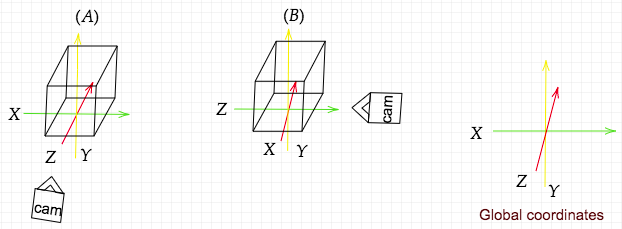
\includegraphics[scale=0.53]{images/campos.png}
\label{campos}
\end{figure}

In graph (A) in \ref{campos}, we see that the camera-view of coordinates align with the global coordinates.The (x,y,z) that go through each object in graph(A) and graph (B) are the view of the axis in reference to the camera. However, if the camera is positioned to the right of the object from our view, as in graph (B), then we say that the camera view of coordinates is not aligned with the global view. We notice in graph (B) that from the camera view, the "global X" is "Y" and vice versa.

Some geometric calculations cannot be preformed if the location measurements are not relative to each other. For example, if we want to calculate the distance between objects the locations must be consistent with one reference point. The camera position is changing and if the location of an object is referenced by the camera's position then we would get locations relative to the changing position of the camera in a time-span. 

To globalize the orientation of the view, measures such as top-down view of a map, or calculating the rotation of the camera from the global center. While the global locations are crucial for measuring the distance, other point-views are also crucial for other purposes. There are three essential coordinate systems to know when working in a 3D environments: 

\textbf{1. World coordinates}(global):  World coordinates(global): The coordinate system that starts at the center of the world; a house in our example. The center of an object in this coordinate system, is then decided by its distance to the center of the world. 

\textbf{camera-view coordinates:} The coordinates from the camera's views. The center of this coordinate system is the position of the camera. The center of the object in this world is defined by its distance to the camera. 

\textbf{3. Local view:} The center of the local view is the object itself. 

The center of all these views is (0,0,0). We described above that the world coordinate system allows us to measure distance between objects in a world map. The camera view is useful if a robot is expected to navigate an environment and describe spatial relations between objects such as "next to", "above". The local view could tell about the size of an object. In particular, the (x,y,z) from a local point of view tell about how far the object stretches from its center where the center is (0,0,0). The local view can be referred to as "radius". 

MatterPort 3D provide the views decribed above. We discuss in more detailed the usage of the object's location in global coordinates and the local view in details in the implementation part.  

\paragraph{Processing geometric data- Methods}

\begin{figure}[H]
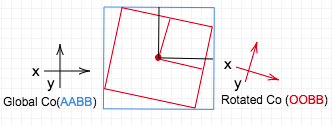
\includegraphics[scale=0.5]{images/A-OB.png}
\label{}
\end{figure}


The geometric information can be classified into two main categories. In a 3D environment we can imagine each object having  a labelling box rotated and oriented around its shape, and other box that bounds the first box with the global coordinates. In figure(X) we see a demonstration of the two boxes in 2d squares. The red box, that is meant to surround an object, is referred to as 'Object Oriented Bounding Box' (OOBB). The coordinates of the OOBB are rotated with rotation of the object (rotated in accordance to the local view). The blue box is referred to as 'Axis Aligned Bounding box'(AABB). The axis of AABB are aligned with global coordinates. 

We extract and save one specific information type of each box. The feature we take is the "radii", or else can be referred to as half-extents. The half-extents (radius) can be helpful in representing the object in different ways.  

We use the radius of the OOBB box to calculate the size of an object. The volume of OOBB gives more precise estimation of the size of the object, as the box is more enclosed around the object.

We use the radius of AABB box to measure the distance of an object to other objects. We can measure the distance between objects in an environment by the distance between their centers. More precise measurements would be to measure the edges or the corners of the object. We get the corners by measuring how far the box stretches(given by radius) from the center.  

Important to mention that we locate entities on a map with coordinate points that are positioned in accordance to one coordinate system (grounded in a the global map). Otherwise the numbers that represent positions would be in-indicative of points in the global view . It is for the latter reasons, the centers (located globally) are helpful to measuring distance-- because they are located on the same coordinate basis.  

The AABB box, provide a straightforward estimation of the positions of the object's shape in the global map. The local view of the AABBs are aligned with world coordinates, therefore allocating its corners globally would only require an estimation of how its radius(given in alliance with world coordinates) stretches from the center.

True that the OOBB corners are better representatives of the objects corners, however, locating the oobb corners in the world map is not simply done by measuring how its radius stretches from the center in the direction of  the global axis as in AABB. The radius of the OOBB is given along its local view axis(its rotation), meanwhile the center point is given in the world axis. Thus, locating the positions of the OOBB, using the same radius-length measure, would require adjusting the radius to the direction of its rotation. Therefore, the global-alignment characteristic of the aabb provides a direct way to locating its edges.  


The corners of the OOBB would be the most precise representation of the corners of an object. 



\subsubsection{EQA (Task Dataset)}

(More information to include-- 1. How they filter out questions based on entropy, and how they filter out objects based on size..2.How many unique question there is. 3. Explain more thoroughly how the singleton(object,room) works) 

The question-answer data-set contains three types of questions.
Each question in the detest is a function that can be executed in the environment to give an answer. More in section (3.2)
\begin{figure}[H]

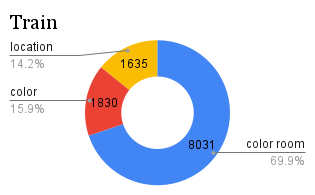
\includegraphics[scale=0.45]{images/Train.png}
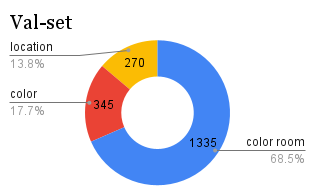
\includegraphics[scale=0.45]{images/Val-set.png}
\end{figure}

%\begin{figure}
%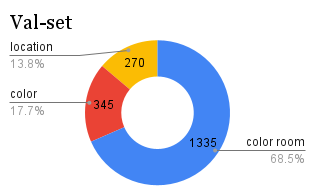
\includegraphics[scale=0.45]{images/Val-set.png}
%\end{figure}


(To include the number of unique questions here )
There is a total 11496 questions in the train split and 1950 questions in the val split. As seen in figure (5),in the train split there are 1830 questions "color" type, 8031 of "color room"  and "1635" of location type. For the validation split there are 1335 "color room" questions, 345 "color" questions, and 270 "location" questions. 



Each question-type is generated in a string template.The templates are as the following:

\textbf{- color room} template: "what color is <obj> in  <room>?": In these questions the agent needs to find the room in question and look for the object and answer the question. For the agent's to be successful at reaching its target, it needs to know the difference between rooms, and objects, as by implicitly recognizing that a certain room is a living-room, not a bathroom and such.  

\textbf{- color} template: "what color is <obj>". The difference between "color" type and "color room" is that no room is specified in the "color" type of question. In "color" type the agent needs to figure out where to look by itself. For example, "what color is the fridge?", the robot needs to implicitly figure that the fridges are usually in the kitchen and navigate to the kitchen to answer the question. In other cases, the object could be in the vicinity of the robot's starting point, so that it all it needs to do is to look around. 

\textbf{- location} template: "What <room> is the <obj> located in". 

\paragraph{Querable objects and rooms}

The questions ask about 50 unique objects. \cite{embodiedqa} in (page 4) describe the process of object and room selection for question generation.The following quoted from (page 4): 

"select(objects)->singleton(objects)->query(location)"

The above represents the steps taken for finding object and location to fill in the questions template. select(objects) is a function that collects all the objects in the house. singleton(objects), filter out an object that occurs only once in the house; query(location) finds the location of the object.However, this applies to the old dataset in SUNCG.

In EQA-MP3D, the object in question is not unique to the house but to the room. The latter means that for an object to be selected for a question, there need to be only one instance of that object existent in the room. The reason for this is to avoid ambiguity, and not to confuse the agent if there happen to be more instances of the same object in the room. 

we observe that all the objects that the robot is asked about in testing have occurred in the training questions. While it has been mentioned earlier that the robot is tested in different scenes from the scenes it was trained on, similar objects from the training co-occur in the testing. The latter means, in particular, that the robot is unfamiliar to the test scenes but familiar with all the objects that are being asked about in the test. This information is also stated in \cite{eqa_matterport}. 


\paragraph{Structure}

\begin{figure}[H]
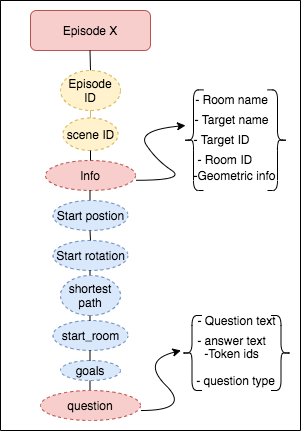
\includegraphics[scale=0.5]{images/episode1.png}
\label{fig:episode}
\caption{}
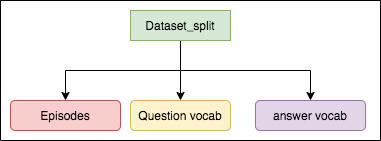
\includegraphics[scale=0.5]{images/datasplit1.png}
\label{fig:datasplit}
\caption{}
\end{figure}

In figure (x) we see the top structure of the val and test. \textit{Episodes} refer to each question-function in the data-set split. \textit{Question vocab} and \textit{answer vocab} contain the same elements as dictionary keys. The elements are: [word list,stoi,itos,num vocab,pad token].

"Question vocab" and "answer vocab" in the "train" and "val" are identical to each other. When using each split of the dataset, the answer-tokens that are considered are the ones contained within the episodes instead of the word-lists mentioned above. 

Each question-sample is an episode that consist of multiple layer information. The structure of one episode of all the "episodes" is as seen in figure(x). We describe the elements of an episode in the following:  

\textbf{House ID}: The house ID given by the house ids in MatterPort3D.
\textbf{Episode ID}: The episode index in the range of the split's length. \hspace{1.5cm}
\textbf{Info}: This element contains all the information about the the object and room in a question. The information is structured as such: 

Information about the traget-object is the first layer within "info": 

\textit{centroid}: The center of the object's box in the global coordinates. Box is the area that labels  the object. When the center is globally oriented we would refer to this center and box as Axis-aligned bounding box(AABB), which means that (x,y,z) axis of the center are aligned with global coordinates. 

\textit{radi}: It tells how far the box (object) stretches from its center one direction of each axis. The value of radii is relative to the object itself (from the local view), where the center is zero. If we have, for example a radi of (2,1,4), this means that the object's box stretches +2 and -2 from the center on the x axis. The boundaries of the object's box relative to itself is referred to as object oriented bounding box (OOB). 

\textit{level}: at which level-floor of the house  is the object located in. 

\textit{room-id}, \textit{room name},\textit{obj Id},\textit{room name} : Room ID, room name and object ID as given by semantic annotation in  Matterport3D. Many of the objects are re-named, mostly names in hyponymes changed to hypernym category such as: round-sofa, l-shaped sofa changed to their hypernym category "sofa". 

The second layer is information about the room: 

Information about the room is similar to the type of information given for the objects. Th information is \textit{floor-level}, \textit{room-id}, \textit{room name},

Final layer consist of a "question-meta" which includes the color of the object. This section also includes question-entropy ..... 

The elements that are marked in blue in figure(x) are navigation-related material. 

\textbf{start position}: The start positions are all unique. For each unique question in the data set there is fifteen different starting position. 

\textbf{rotations}: This is the rotations that the agent have to do while navigating. It stands as supplementary information for the shortest path 

\textbf{goals}: Goals are the destinations that the agent should reach in navigation. The goals stand for the possible view points from where the the target object can be looked at by the robot. Each view point consist of geometric position and the rotation toward the target object respective to the position. 

%\begin{figure}
%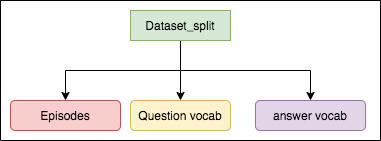
\includegraphics[scale=0.5]{images/datasplit1.png}
%\end{figure}



\paragraph{expirement}


The idea is to extend the question asked for the agent. The two types of questions are size and spatial. The process of question extension includes using information from the initial EQA-v1  dataset, which consists of color, color-room, and location questions. Each question sample has a target object with corresponded information as object ID, room ID, Scene ID, question(token-ids and text), and shortest path. We pick the object and the room ID for every question sample to extract the rest of the information about the other things in the room. The extracted information is the volumes of the objects and the 




\newpage

\section{Task 1- Question Generation}
\label{sec:task1}
\subsection{ Overview Extending Dataset}

The idea is to include more questions about the same objects and the scenes found in EQA-v1. The question generation copies the EQA data-set and modify the so called-episodes in it. The episodes, as mentioned in previous sections, are executable functions when inserted in an environment they yield an answer. The scenes denote the visual scene of the destination goal of the a navigational episode. The system learns to reach its navigational goal by a shortest path included in each EQA-V1 episode. Our new questions use the same shortest path found in EQA-V1. 

This project consist of two major module-components. The first module is a parser that does data extraction, and acts as a processor for raw data by transforming into usable geometric information for generating question-answers. The second module is the question-answer generator. This chapter describes the projects construct and the usage of each part of it.  



\subsection{First module- Data parser}

Our house parser consist of two classes. The first class is a class that parses the houses into a structural data. The second is functional class we use to find near objects close to a target object. The latter class is used 

The experiment include used two different ways for annotation extraction. The first source-method is the raw annotations given in the 'house files' of the MP3D data-set. The second method uses Habitat's simulator and sensors. The annotations extracted from the sensors in the Habitat's simulated environments provide more computed information and slightly different raw data MP3D annotations; In particular, some object names are different, but the rest of information, such as object ids and location-centers, is consistent with the annotation of the MP3D. 

In the existing generated question-answers data-set we use the data extracted from the Habitat semantic sensors. The main reason for choosing Habitat's semantic sensors is because they provide a computed geometric information of the objects such as the location of an object within an Axis Oriented Bounding Box (We elaborate on this term in the coming section). An additional important reason for this choice of extraction is that some of  objects names output-ed by the sensors are aligning with the names found in the original EQA-V1 data-set. For example, object names in MP3D such as l-shaped sofa and rounded-sofa are transformed, in Habitat's sensor, into their Hypernym category 'sofa'. Choosing object names that are aligning with names found EQA-v1, is helpful for having the overall data consistent with each other when we emerge our generated questions with EQA-V1. 

The second major component - get close distances 


\subsubsection{Annotations from MP3D files}


We extract two types of raw information from each object's line of annotation found in the house files in Matter-port. Lines mentioned erlier: [px py pz  a0x a0y a0z  a1x a1y a1z  r0 r1 r2 0 0 0 0 0 0 0 0 ] 

First we take the obj and room indexes (ids). Second is the [px py pz] and where we categorize it as the center of the object's box. Third is the [r0 r1 r2] (radius-half-extent).

we structure the data in a form that the annotation of a house begins with the first level in it, followed by the rooms and objects in each room as: house 1 [{level1:room1[bedroom]:(obj1:bed,obj2:..),room2:(obj..)},, {level2:......} ]  

\subsubsection{Annotation extraction using from Habitat's sensors}

Our final choice for extracting semantic annotations is Habitat's simulator. Our annotation's parser of the houses uses the sensors with configuration provided by the habitat platform \footnote{url{https://aihabitat.org/docs/habitat-lab/habitat-sim-demo.html#scene-semantic-annotations}.}. The configurations include the settings such as the scene, the height and width of the sensors, and the types of sensors to include. color sensor, semantic sensor and depth sensors are used. 

Once we simulate the environment, the sensors output the annotations of a house(scene) as an object. We iterate through the object to obtain information about the levels, rooms, and the objects in the rooms. We freeze the simulator once the annotations' object of one environment is outputted, then repeat the process for the other environments. 

The data about the an environment's annotations include a calculated geometric information. The sensors in the simulator gives an advantage by calculating the sizes of both the AABB and the OOBB. We use the sizes of the OOBB and AABB, to further obtain more specific information about the object's boxes. 


\begin{figure}[H]
\centering
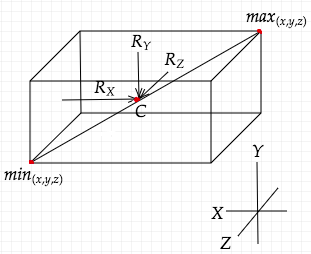
\includegraphics[scale=0.5]{images/Geoinfo.png}
\caption{Min and Max of an Axis Orients bounding box}
\label{fig:aabb}
\end{figure}


We make calculations from the data we extract in order to obtain other necessary info for generating question. Important to mention, the geometric points extracted by habitat's simulator, such as centers of the boxes and the sizes of the boxes' sizes, are represented in 3D data where the  x is the length, y is the width, and z is the height. 

The first calculation is finding the 'min' and 'max' of a bounding box given an object's center and length of its sides on(x,y,z). In figure \ref{fig:aabb} we see visual illustration of the extracted and calculated data. The min represents the corner of a box that has the lowest value of (x,y,z) and max is the corner with largest value for (x,y,z). Other way to put it, the min represents the corner point in the minus direction from the center in all the axis , and max is the corner on the positive direction from the center in all axis. 
%$\displaystyle
The given size of the box is from the min point to the max point with a 3d value (x,y,z). To get each of the points we first get the half extent of the size such as: \begin{math} Half\ extent\ =(x,y,z) /2\ \end{math}. half extent or (radius) is the point from the center to either the min or max. 

The 'min' is the point stretched by the length of the half extent in the negative direction, and 'max' is the stretch to the positive as the following:   \\ 
\begin{math}
Min\ point\ =\ C\ -\ \vec{H} \ \ =\ ( x\_{1} +x\_{2} ,y\_{1} +y\_{2} ,z\_{1} +z\_{2}{}) \  \\
Max\ point\ =\ C\ +\ \vec{H} \ \ =\ ( x\_{1} -x\_{2} ,y\_{1} -y\_{2} ,z\_{1} -z\_{2}{}) \ 
\end{math}

The min and max help us in define spatial relations among objects. How we use them is explained in the coming sections.

We use the OOBB sizes for calculating the sizes of the objects. We consider the size as the volume of the box which is the length multiplied with the height and width. In our case the length is the x value, width is the y value and z is the height, then  the calculated volume of a box is \begin{math} X\ x\ Y\ x\ Z \end{math}. 


We structure the annotations and save them in a file. The structure of the data consist of a dictionary storing the data in a hierarchical way. At the top part is the house id, then rooms in the house, then the objects in the house. Each object stored by id, contains the min and max value of its box, size of its aabb, its name, room name and id where its located, and the level id where the room is located. Storing the annotations this way allows to access all the objects in a room through the scene id and room id. 

 We store the calculated volume of each object in all the houses and store it in a second file. The volumes of objects are stored by their object category. In the volumes file, we find the volumes of all the objects in all of the houses stored in a dictionary, each key represents a category such as 'sofa' with values of the volumes of this object type. The point here is to obtain data on the sizes of each object type. We use this information for finding ground truth answers about for the size questions.  
 

\subsubsection{Second class - Distance and size calculator}

The main functionality of this class is to find a spatial relation between pairs of objects in a room. It takes as an argument scene and room id and uses this information to access the objects in a room from the parsed houses files. 

It outputs three types of spatial relations between a pair of objects. The pairs spatial relation is specified by whether an object is 'on' , 'next' or in unspecified 'close' distance to a second object. The pairs are organized in a dictionary, one key for each spatial relation. This information is used for generating positive spatial questions. 

The spatial relations mentioned above are measured by calculating the distance between the corners of the objects' bounding boxes along certain dimensions. The corners obtained using the 'min' and 'max'. If we iterate over the Min(x,y,z) and Max(x,y,z) we get the other six corners of the box. Figure \ref{fig:box_points} illustrates the eight corners, the view point of the cube is rotated to the right for the sake of viewing all the points in the cube. If we move our point of view directly in front of the cube as if  we are facing the square GHED,  the points A and H would seem to be lying on a straight line. Lying on the same straight line, for example, means the point A and H are located on the same points in the x-axis, and so one for the other parallel points .\begin{figure}[H]
\centering
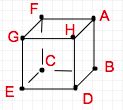
\includegraphics{images/cornerPoints.png} %[scale=0.5]
\caption{}
\label{fig:box_points}
\end{figure} 

We get the rest of points from the Min and Max of an AABB for the reason that AABB's are not rotated and aligning with the global view. To express it better, we image the global point of view of the AABBS as a view facing a group of adjusted and not rotated boxes. 

For our example in figure \ref{fig:box_points}, the values of the six corners of the box found from the Max and Min in addition to the corners of the Min and Max would be as such: 

$\begin{array}{l}
A\ =( x_{max} ,Y_{max,} Z_{max}) ,F=\ ( x_{min} ,Y_{max,} Z_{max}) ,H\ =\ ( x_{max} ,Y_{min,} Z_{max}) ,\\
B=( x_{max} ,Y_{max,} Z_{min}) ,D=\ ( x_{max} ,Y_{min,} Z_{min}) ,\ C=( x_{min} ,Y_{max,} Z_{min}) ,\\
G=\ ( x_{min} ,Y_{min,} Z_{max}) ,\ E\ =( x_{min} ,Y_{min,} Z_{min})
\end{array}$

  


A visual representations of the corners and their values seen in figure.X 


The definition of each of the mentioned spatial relation , is an approximation of how we define them as humans. Each of the spatial relations are determined given a geometric criteria of distances and positions between objects' corners along the three axis  (x,y,z). 

Two general operations are used in each of the relations. The first one is calculating  the Euclidean distance between two corner points; denoted as the distance between p and q in this formula:  \begin{math}
 d\left( p,q\right)   = \sqrt {\sum _{i=1}^{n}  \left( q_{i}-p_{i}\right)^2 } 
 \end{math}

The corners, depending on the type of relation we want to extract, can be represented as points in  1d, 2d, or 3d. 1D is  when we pick points from one of the axis only. 2D is a point on two axis, and 3D is a point on three axis as the corner examples illustrated earlier. We describe this in more detail in the sections below. The second operation is calculating if one of side of a box on a certain axis is contained within the other. 

\begin{figure}[H]
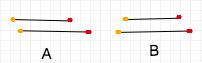
\includegraphics[scale=0.5]{images/contained.png}
\caption{}
\label{fig:contained}
\end{figure}

The calculation if one side is contained within the other relies on defined criteria. The calculation is done in a specific function and  can take as input  corner points on one axis or more. In the drawing \ref{fig:contained} 'A' represents two lines on the 'X' axis where the top part is not contained within the other, an in 'B' the top is contained within the lower line. In this example we determine the 'contain' relation by taking the 'min' represented by the the orange dot and the 'max' doted in red. 

If the min of the upper line is greater than the min of the lower line and the max of the upper line is less than the max of the lower line then the upper line is contained within the lower. Hence the 'min' of the upper line is greater than the 'min' of the lower line because it's more to the right in the positive direction of the 'x' axis. If the previous condition is not satisfied, then the lines are otherwise not contained. 


The operations above are done over different axis for every relation. Below we specify how each of the 'on', 'next to', and 'close' relation is determined between the objects. 

\paragraph{On}



First step is choosing pairs of objects that are closest to each other vertically(on the Z axis). The distance should be less than a 0.5 millimeter thresh hold. The Euclidean distance here is calculated between the 1D points on the Z axis only. Two corner values from each box and any corner match the distance required are picked out. 

\begin{figure}[H]
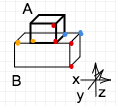
\includegraphics[scale=0.7]{images/on.png}
\caption{}
\label{fig:on}
\end{figure}


The second step consist of a group of conditions that the pair of objects need to meet in order to be considered on each other. The first condition is that the vertical sides, the line from Zmin to Zmax, of the boxes are not contained within each other. The Zmin-Zmax lines of every object box are the lines between the two red dots in box A ans B in the illustration \ref{fig:on}. Otherwise if the lines on the Z axis are contained it would mean one object is inside the other. 

The second condition is that the horizontal line of one of the boxes is contained within each other.The horizontal lines in the illustration are from the Orange to the red points in each box. The lines on the y axis from the red to the blue points should also be contained. 

The final step is deciding which object is on the top of the other. The pair of objects are passed to a function that see which Zmin-Zmax has greater value. The object on the top should be in the upward positive direction. 


\paragraph{next to}


\begin{figure}[H]
\centering
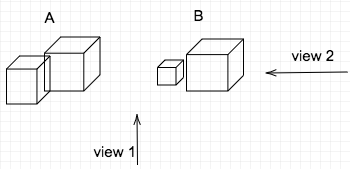
\includegraphics[scale=0.5]{images/Nextview.png}
\caption{}
\label{fig:next}
\end{figure}


A pair of objects next to each other have to have a distance not greater than 0.1 meters on the X and Y axis. The distance here is calculated for 2D corner points, this means the distance is calculated for four corners (min and max front and back).

The pairs should not have contained sides in neither the x nor the y axis. In this condition a pair of objects next to each other would like illustration A in \ref{fig:next}. This is might a bit different from what we consider next to each other as humans. We might imagine a typical next to pair as illustration B seen from view 1.

However, the choice of having 'next to' pairs not contained with each other is due to considerations of the view point. From view 1 the pair(B) seem next to each other but from view 2 they would not. In pair(B) from view 2, one object would be behind the other and likely hidden. So if view 1 is the global view and we pair the objects as in (B), seen as next to in view 1, the robot might enter the scene from view 2 and it would be wrong to refer to the pair as next to each other. However, if the 'next to' pairs are assigned as in illustration (A), the pair would be still visible in whichever view, and positioned proper enough to be referred to as next to each other. 

Finally the pair must have their lines contained on the Z axis. Otherwise, the two objects might satisfy the first condition on the (x,y) but be distant on the z axis, such as one object in the ceiling and the other on the floor. 


\paragraph{close to}

A pair close to each other are a pair who has any of their 3D corners close to each other within a max distance of 0.2 meter. No other conditions required for the pairing of objects close to each other. It can be a close object on, above, below or next to. 

\subsection{Second Module - question generation}


\begin{figure}[H]
\centering
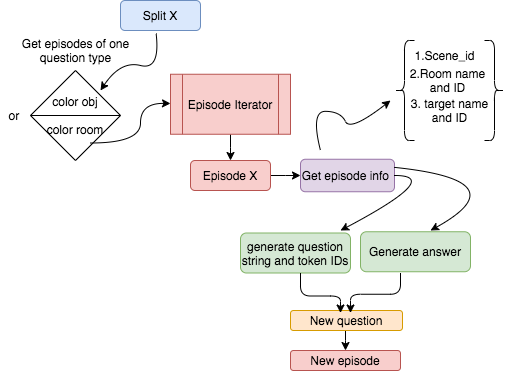
\includegraphics[scale=0.5]{images/generator.png}
\caption{Split generator}
\label{fig:generator}
\end{figure}



 Our question generator generates questions of two types, size and spatial. In order to run the generator, the arguments required are the type of question, path to the val and train splits. 


 The question generator generates questions of one type at the time. Questions with the string "room" in is considered a different type from a question that refers to objects without a room. For example, the question "How big is the table?" has the type "Size", and the question "How big the table in the living-room?" is of type "Size room". In order to generate size questions with and without reference to a room, therefore, requires ruining the code, one separate time for each type. 

The split generator is the core component in the code. It takes a split either train/val and a question-type as arguments. The functionality of the split generator is to turn an EQA v1 split of episodes into a new split of new episodes. In figure \ref{fig:generator} we see an illustration of the workflow of the split generator. The five general steps is filtering(uncolored rotated square), iterator(red rectangle), episode parser (pink rectangle),  QA generator (the green rectangles), and  episode wrapper (the bottom yellow rectangle- inputs QA and outputs episode )  

The filter returns a set of question-episodes of one type only. The returned set of questions of a type is dependent on the question type given to generate. For example, if the input is to generate questions of 'size-room', 'how big is the sofa in the room', we take only the questions of "color-room" type. 

The filtered set is passed to an iterator. Each iteration passes one episode from EQA-v1 to a parser. The parser function in the iterator extract information, such as the object name and id, scene ID and room ID, from the EQA-V1 episode. 

The parsed information is passed to a QA generator. The QA generator is better described  as a group functions of the split-generator that are conditioned differently dependent on the question type. The answer generation function is, however, a different function for each question type.  

 The general idea for generating QA of any type relies on two straightforward steps. First, generating a ground-truth answer for the given question, which is the most important stage in the generation process as it requires calculating values from the data in the houses. Second step generating a question string and token ID's.

The  final step consists of inserting the new question with the corresponding geometric information, and structuring them into an executable function.  We call a QA sample an episode when the section of the episode seen in figure \ref{fig:episode} are filled with the new QA and the other the corresponding information. 

Our question generation can be described as generating one question for every “shortest path” there is. The idea of transforming  an episode from EQA into a new one is based on using the starting position and the 'shortest path' found in them. Having more questions for each shortest path is equivalent to having multiple questions about the same scene. 

\begin{figure}[H]
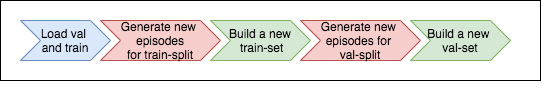
\includegraphics[scale=0.5]{images/stages.png}
\caption{Split generator (The top part of the code)}
\label{fig:stages}
\end{figure}


The top most part of the code (the data-set generator), illustrated in figure\ref{fig:stages} , passes the train and val to the split generator at different time-stamps. The reason for generating the two splits in two different stages is to keep track of the number of question-answers generated for each split. Emerging the two splits and splitting them randomly at the end might create and imbalance between the  answers in each split. The current code controls the distribution of answers in the train and val sets. Otherwise, leaving the type of answers uncontrolled would leave a bias towards one answer over the other. 

Once a split of episodes is generated it's passed to loader function. The loader function inserts the answer and question vocab to finalize the data-set in the form seen in figure 2.2

 In the coming two sub-section we describe in detail how the QA generators for the size and spatial questions work. 

\subsubsection{size-questions}

Size questions are generated through three steps. The first step is generating a ground truth answer about the size of the the target-object found in EQA-V1 episode. There three possible answers are  Big, Small, and Medium. The second step is generating a question string and token ids. The final step consist of filling the question-answer in an episode form, with shortest path and the rest of object's info from the original EQA-v1 episode, as described in the previous section. 

\subsubsection{Size answer} 

The size answer is generated in a function referred to as "GetsizeAnswer". This function takes as an argument the target-object's name and the size of its box and returns an answer about its size. The function calculates the volume of the target object in a similar way as the rest of the sizes of the objects. Volume of the OOBB = W x L x H. The next step in the function is to compare the size of the target to the sizes of the objects of its type.

The relative size is determined by its deviation from the standard of its type. As mentioned earlier the sizes of all objects are stored by type in a file. We pick the volumes of the object's type and calculate the mean size and the standard deviation of all the the sizes from the mean. The standard deviation denoted below: 

\[ s = \sqrt{\frac{1}{N-1} \sum_{i=1}^N (x_i - \overline{x})^2} 
\]

The answer is 'small' if the objects' size is smaller the mean size of its type minus the standard deviation,  'big' if the size is larger the median + the standard deviation, and middle if the size of the object is within the standard deviation added and subtracted from median. 

We control the answers' distribution. We observe that a majority of objects have a medium size given the standard of their type. In order to avoid bias towards the 'medium' answer, we restrict the number of QA with medium answer. We keep track of how many QA with medium answers has been generated and when the number reaches a limit we generate None QA that are later filtered out. The limit varies depending on the question type and the split (train or val), and is based on our observation of the answer distribution in the splits. Note that we refer to 'question type' in this example if either the question to be generated is size question with string 'room' such as "color-room" or without. 


\paragraph{question-string}

The question string generator takes a question type, and an object as an argument and returns a complete question string. 

The templates for size questions are as the following: 

size\_obj : 'how big <AUX> the <OBJ> ? \\
size\_room:'how big <AUX>  the <OBJ> in the <ROOM>?'

\subsubsection{spatial-questions}

Generating spatial question takes more complex steps and longer time than generating size questions. Generating a spatial QA requires a coordination with the spatial relation extractor. In addition, spatial questions include the addition of an extra object to the question string, and the insertion of the new object's information into the QA episode. 

Searching for spatial relations of the target object in an EQA episode is the first step taken. We pass the scene an room id to the 'relation' extractor to obtain pairs of objects, within a room,  with a spatial relation between them. The relation extractor returns three types of relational : next, on, or close, if existent within a room. Else it returns a category with empty values. 

The decision of generating a question of one of the mentioned relational categories is dependent on the existent of an object with a spatial relation to the target object. The process of executing a generation command of a question of a spatial type is illustrated in figure \ref{fig:spatial}. If there is an object 'on' the target or a target is on another object, we generate one questions, and similar case if there is an object next to the target object. If there is no 'on' or 'next' relation or either of them is non existent, the criteria for checking if there is a 'close' object is satisfied. If none of the conditions are satisfied a QA with no 'answer' of a random spatial type is generated.   

\begin{figure}[h]
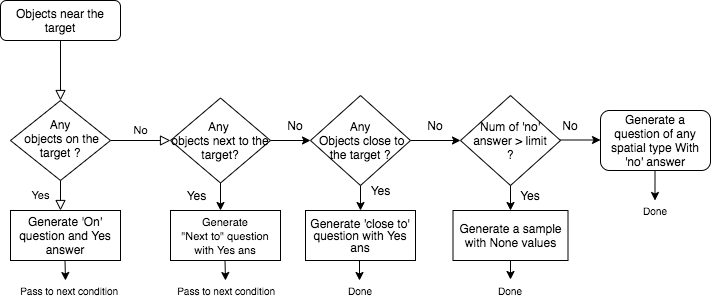
\includegraphics[scale=0.4]{images/spatialconditions.png} %[scale=0.2]
\caption{Decision tree for generating different types of spatial questions}
\label{fig:spatial}
\end{figure}

A QA with positive spatial answer has a 'yes' answer, and 'no' if a relation is non existent. The decision tree as seen \label{fig:spatial} leverages positive QA for the reason that we observe that the no-relation instances outnumber the positive ones. The final condition, we even control the number of QA with 'no' answer by generating a None QA if the number of generated QA with no answer reaches a limit. The QAs' with None values are later filtered out.

Within this decision structure, for each 'shortest path' in an EQA episode, there is a possibility for generating from one to two spatial questions of different spatial type. 

The process of generating a spatial question includes the addition of information about two objects. An episode/question generator, a group of functions, adjust itself to a spatial question generation if certain arguments are given to it. These arguments are seen in the input section  in the illustration in fig \ref{fig:spatialGen}. Such as potential  object type, spatial question type, and all object in a room 

\begin{figure}[h]
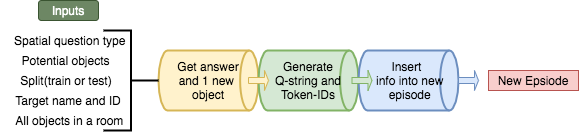
\includegraphics[scale=0.4]{images/spatialGenerator.png} %[scale=0.2]
\caption{Structure of spatial questions generator}
\label{fig:spatialGen}
\end{figure}

All the inputs seen in \ref{fig:spatialGen} are required to generate an answer from a function called "GetSpatialAnswer". All objects in a room are needed for generating "no" answer. In case of generating a "no" answer the "GetSpatialAnswer" function picks a random object fro the houses that is not in the room. The reason of excluding objects in the room from the selection of a random object for a negative QA is to help us in the validation process, such as we would know if the robot answer 'yes' to a QA with 'no' as ground truth that it's due to bias rather than he robot recognizing the object in the scene. 

A selected object of potential objects and the type of spatial question are required arguments for generating spatial question string and token ids. 

The last part in blue is conditioned by the type of answer, if it's 'yes' or 'no'. If the answer is yes, geometric information of the target object's pair is passed to it to insert it in the episode. If the answer is 'no', no additional information is added to the episode beside the information of the target object found at the end of the shortest path. 
\paragraph{Question strings}

To generate a spatial question string, the string generator takes as an argument the question type such as "spatial\_room" and and spatial relation type such as "on", "next" or "close". The string templates are the following: 

'<AUX> there <ARTICLE> <OBJ1> close to the <OBJ> in the <ROOM>?'/\\
'<AUX> there <ARTICLE>  <OBJ1> next to the <OBJ> in the <ROOM>?' \\
'<AUX>  there <ARTICLE> <OBJ1> on the <OBJ> in the <ROOM>?\\
'<AUX> there <ARTICLE> <OBJ1> close to the <OBJ>?',\\
'<AUX>  there <ARTICLE> <OBJ1> next to the <OBJ> ?',\\
'<AUX>  there <ARTICLE> <OBJ1> on the <OBJ>?'


\subsection{Results}

\subsubsection{Total number of generated questions}

\begin{figure}[H]
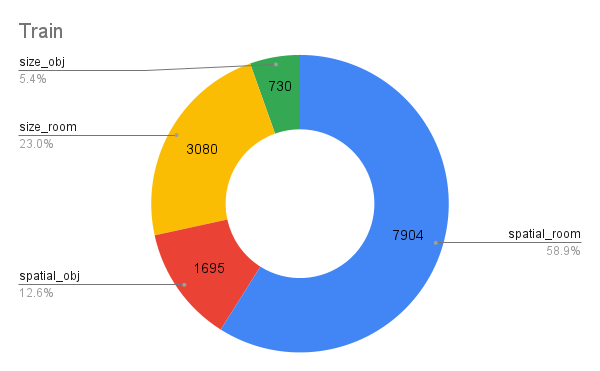
\includegraphics[scale=0.25]{images/GenTrain.png}
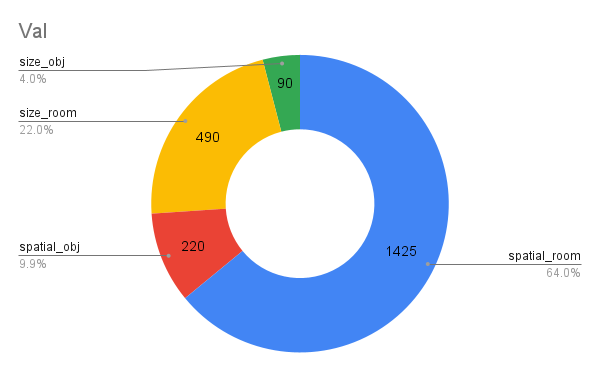
\includegraphics[scale=0.25]{images/GenVal.png}
\caption{}
\label{fig:questionGen}
\end{figure}

We generate a total of 13 409 question for train and 2 335 questions for validation.  In figure \ref{questionGen} questions of size\_room and spatial\_room refer to questions that contains a reference to a room, such as 'How big is the bed in the bedroom?'. Questions of spatial\_obj or size\_obj type are questions with a reference to object only, such as "Is there a chair next to the table?". 

\subsubsection{Answers distribution}

\paragraph{Answers distribution of spatial questions}

\begin{figure}[H]
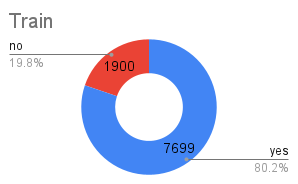
\includegraphics[scale=0.45]{latex/images/TrAnSp.png}
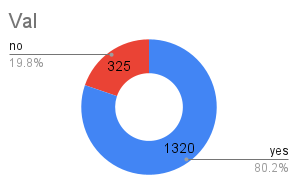
\includegraphics[scale=0.45]{latex/images/VlAnSp.png}
\label{fig:AnsDist}
\caption{}
\end{figure}

The majority of answers for the spatial questions are positive "yes" as seen in figure \ref{fig:AnsDist}. This imbalanced distribution is an intended outcome. The motivation behind this intention is based on an idea, formulated by \cite{regier1996human}, of learning of positive samples only. The argument behind this approach to learning  is inspired from a cognitive theory of human's first acquisition of language. The theory is  based on the premise that humans tend to learn spatial relations from positive evidence instead of non existent instances.

\paragraph{Answers distribution of size questions}

\begin{figure}[H]
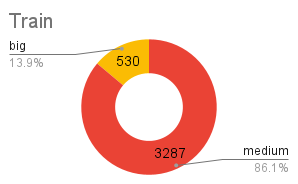
\includegraphics[scale=0.45]{latex/images/TrAnSi.png}
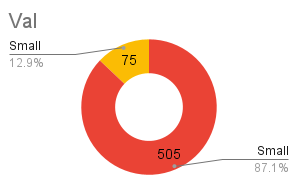
\includegraphics[scale=0.45]{latex/images/VlAnSi.png}
\caption{}
\label{fig:AnsDist}
\end{figure}

The outcomes of generating size questions resulted with zero samples of "small" answer and a majority of 'medium' answer as seen in figure \ref{fig:AnsDist}. In the QA generator, we intended to limit the question-answers with "Medium" answer based on an observation of their dominance. However, limiting the 'medium' answers more than the presented numbers would have resulted in a very few question-answers of size type. An insignificant proportion of size questions was insufficient for training the model . We decided to keep the size questions with their imbalanced distribution, despite knowing that this linguistic bias might hinder the learning outcomes.  

\subsubsection{Discussion}

Our question-answer generation is very dependent on the objects and the shortest paths found in EQA-V1 data-set. The geometric information such as  starting positions and shortest paths are required material for extracting scenes training and testing the VQA model. To be only dependent on the objects found in the EQA restricts our choice over the QA that we could generate. The most prominent limitation we see in the generated questions is the inability to control the answer distribution for size questions. None of the target object's found in EQA V1 turned to be of a small size, based on the criteria we establish for determining an object's size. 

The description of sizes is paradoxical. A well established paradox, in philosophy


Topic sentence: we add spatial questions for the goal of .... deespite haing lingustic bias? 

Evaluation depending on no answers


Our choice to include size and spatial questions is motivated by the belief of the importance of spatial language to cognition. (\cite{landau1993whence}) in “spatial language and spatial cognition” states that the human first acquisition of linguistic names of objects in the physical world is associated with establishing a geometric representation of what defines them. In particular, the conceptual identification of an object might be defined within a spatial relation to other entities, and the image we mentally construct of a concrete noun of a physical property, may appear in the form of its shape.

The annswer 

Our question-answer generation is very dependent on the "shortest paths" in EQA-V1 data-set and the objects they lead to.  






\section{Task 2- Question Asking}
\label{sec:task2}


\subsection{Training}




\subsection{Evaluating}

\begin{figure}[H]
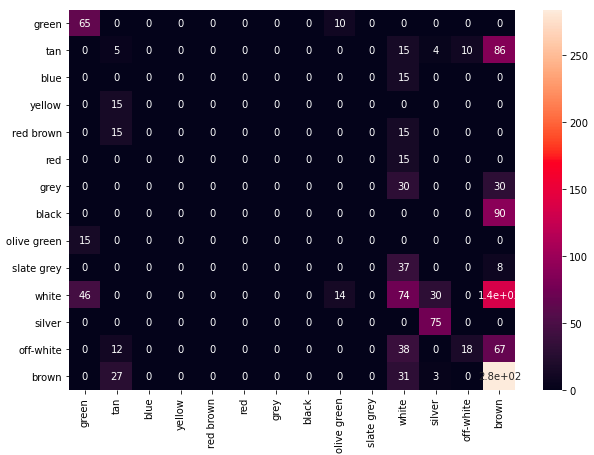
\includegraphics[scale=0.45]{latex/images/Heatmapbefore.png}
\label{fig:Heatmapbefore}
\caption{Predictions of color questions before training with new questions}
\end{figure}

\begin{figure}[H]
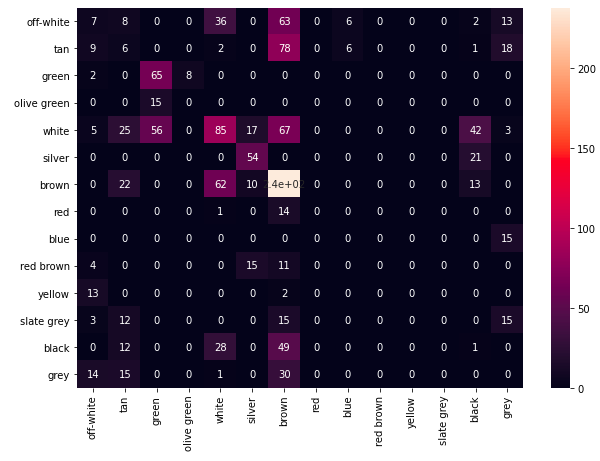
\includegraphics[scale=0.45]{latex/images/HeatmapAfter.png}
\label{fig:HeatmapAfter}
\caption{Predictions of color questions After training with new questions}
\end{figure}

\begin{figure}[H]
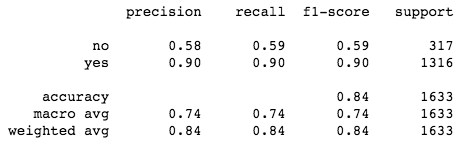
\includegraphics[scale=0.45]{latex/images/spatialscore.png}
\label{fig:HeatmapAfter}
\caption{Scores for spatial questions}
\end{figure}



\subsection{Discussion}

We should treat neural models as a theory or brain that is applicable and functional for every task scenario \cite{regier1996human}  



However, color questions could get more complex as "people employ compositional color descriptions to express meanings not covered by basic terms, such as greenish-blue" \cite{monroe2016learning}. It would be shallow to assume that color questions are simplistic, especially if we expect the system to answer colors beyond the basic color terms like "green" and "red." 

\cite{monroe2017colors}


intersective compostionality: intersective compositionality is when two words which one is attributed to the meaning of the other "brown bear" where it means a bear that is brown-[brown and bear] 

non-intersective compostionality: non-intersective is one word does not modify the second, such as [Teddy bear]. 'Teddy bear' cannot be mean a bear that is 'Teddy', 'Teddy' is not an attribute of a bear so not [Teddy + bear]. Teddy + bear is instead a different entity with a different perceptual meaning. 

\cite{larsson-2017-compositionality} 


\addcontentsline{toc}{section}{References}
\bibliography{references}

\newpage
\section{Appendices}

\end{document}


